% PaperLens: IEEE conference paper (two columns).
% Build: pdflatex paperlens && bibtex paperlens && pdflatex paperlens && pdflatex paperlens
% Lines marked TEAM need the team's input before submission.
\documentclass[conference]{IEEEtran}
\IEEEoverridecommandlockouts

\usepackage{cite}
\usepackage{amsmath,amssymb,amsfonts}
\usepackage{graphicx}
\usepackage{booktabs}
\usepackage{multirow}
\usepackage{makecell}
\usepackage{array}
\usepackage{xcolor}
\usepackage{tikz}
\usetikzlibrary{positioning,arrows.meta,fit,backgrounds}
\usepackage[hidelinks]{hyperref}
\usepackage{url}

\newcommand{\yes}{$\checkmark$}
\newcommand{\no}{--}
\newcommand{\part}{($\checkmark$)}

\begin{document}

\title{PaperLens: Evidence-Grounded, Reproducibility-Aware Analysis of Research Papers with a Free-Tier Language Model}

% TEAM: names, e-mails and affiliation of every author.
\author{
\IEEEauthorblockN{Author One, Author Two, Author Three, Author Four}
\IEEEauthorblockA{\textit{Department of Computer Engineering} \\
\textit{Sardar Patel Institute of Technology}, Mumbai, India \\
\{first.last\}@spit.ac.in}
}

\maketitle

\begin{abstract}
Large language models (LLMs) can summarise a research paper in seconds, but the facts they
report come without evidence. For research, an invented number is worse than none. We present
\emph{PaperLens}, a system that takes a paper (PDF or link) and returns a structured breakdown
in which every extracted item carries the verbatim sentence it came from. Python locates
that sentence in the PDF and highlights it, and a second check judges whether it supports
the item. On top of this grounded extraction, PaperLens scores reproducibility against a
21-item checklist, verifies numeric claims against the paper's own results tables,
discovers the paper's code repository and compares its settings with the paper by static
analysis, and offers page-cited chat, a notation glossary, a citation graph, a draft review
and a multi-paper comparison. The design follows one rule: \emph{the LLM extracts and
Python decides}. Every score, delta and verdict is computed deterministically, and the
whole system runs on the free tier of a commercial LLM API. On a 10-paper gold set,
extraction reaches a core-field F1 of 0.72 with precision between 0.79 and 1.00 per field.
Every extracted hyperparameter whose name matched the gold had the correct value, and 80\%
of extracted items are verified against the paper. Requiring a located quote lowers the
hallucination rate from 10\% to 2\%, and adding the support check lowers it to 0\%, at a
cost in recall that we quantify. We release the system, the evaluation package and an
annotation guide.
\end{abstract}

\begin{IEEEkeywords}
scientific information extraction, grounding, attribution, reproducibility, large language
models, document parsing, claim verification
\end{IEEEkeywords}

% =========================================================================================
\section{Introduction}

Reading a research paper well takes one to three hours, and much of that time is spent
finding the same facts: the datasets, baselines, metrics, hyperparameters, compute and
limitations. Judging whether the work can be reproduced is harder still. Surveys of the AI
literature found that no sampled paper documented every factor needed for
reproduction~\cite{gundersen2018state}. An attempt to re-implement 255 papers without
their code succeeded only about two times in three~\cite{raff2019step}. Released code
does not settle the question either, because it often uses settings other than those
reported~\cite{pineau2021improving,collberg2016repeatability}.

LLMs are an obvious aid, but their output is fluent and unattributed, and they hallucinate
facts~\cite{ji2023hallucination}. Attribution research shows that generated statements must
be checked against an identified source to be trusted~\cite{rashkin2023ais,gao2023alce}.
For scientific use, where a wrong learning rate silently ruins a replication, unverifiable
output is of little value.

We present \emph{PaperLens}, built around a single principle: \textbf{the LLM extracts, and
Python decides}. The LLM's only job is to read text and return schema-validated items, each
with a verbatim quote. Deterministic code does everything else. It locates every quote in
the PDF, scores reproducibility, matches claims to table cells and recomputes their deltas,
compares the paper's hyperparameters with the code, and draws every verdict. The system
runs on the free tier of the Gemini API~\cite{gemini2023}, so every design choice also
minimises the number of LLM calls.

Our contributions are:
\begin{enumerate}
\item An end-to-end system that parses a paper with layout coordinates and extracts a fixed
  schema. Every item carries evidence that is located in the PDF and checked for support,
  and items that cannot be verified are labelled rather than dropped.
\item Three deterministic checks built on the extraction: a reproducibility scorecard, a
  claim verifier that recomputes claimed differences from parsed tables, and a static
  paper-vs-code comparison that never executes repository code.
\item An evaluation package with a documented matching scheme, a gold set over ten widely
  used ML papers, and three ablations that need no LLM calls: evidence policy, parser and
  retrieval.
\item An honest assessment. Precision is high on every core field, the main weakness is
  recall on hyperparameters and tasks, and our reference annotations were produced with
  LLM assistance.
\end{enumerate}

% =========================================================================================
\section{Related Work}

\subsection{Scientific information extraction}
Entity and relation extraction from papers has been studied with dedicated datasets:
SciERC for entities, relations and coreference~\cite{luan2018sciierc}, SciREX for
document-level task/dataset/metric/method relations~\cite{jain2020scirex}, and the
leaderboard-construction work of Hou et al.~\cite{hou2019tdms}. AxCell extracts results
from machine-learning papers, using table segmentation~\cite{kardas2020axcell}. These systems
rely on fine-tuned encoders such as SciBERT~\cite{beltagy2019scibert}. Dagdelen et al.\ fine-tune
LLMs for joint named-entity and relation extraction that outputs structured JSON for
materials science~\cite{dagdelen2024structured}. PaperLens differs in two ways. It uses a
general-purpose LLM without fine-tuning, and it makes evidence a first-class output that is
checked against the source rather than an optional by-product.

\subsection{Parsing scientific PDFs}
GROBID turns PDFs into structured TEI with sections, references and
coordinates~\cite{lopez2009grobid}, and it underlies corpora such as
S2ORC~\cite{lo2020s2orc}. Nougat converts page images to markup with a vision
transformer~\cite{blecher2024nougat}, and Docling combines layout analysis with table
structure recognition~\cite{auer2024docling}. Table structure recognition has its own
benchmarks~\cite{zhong2020pubtabnet,smock2022pubtables}. We found GROBID's table grids to be
unreliable on our papers, so PaperLens rebuilds each grid from the PDF's word positions and
uses GROBID for structure, sentences and citations (Section~\ref{sec:parse}).

\subsection{Grounded generation and attribution}
Retrieval-augmented generation conditions an LLM on retrieved passages~\cite{lewis2020rag}.
ALCE evaluates generated text whose statements cite their sources~\cite{gao2023alce}, and
the AIS framework defines when a statement is attributable to an identified
source~\cite{rashkin2023ais}. FActScore breaks text into atomic facts and checks each against
a knowledge source~\cite{min2023factscore}, while SelfCheckGPT detects hallucinations
without external resources~\cite{manakul2023selfcheckgpt}. Long contexts are used
unevenly by LLMs~\cite{liu2024lost}, which motivates our per-section extraction.
PaperLens applies the attribution idea at the level of single extracted items and enforces
it in code. A quote is accepted only if a fuzzy string match~\cite{levenshtein1966} finds it
in the parsed paper.

\subsection{Question answering and reading assistants}
Qasper anchors information-seeking questions in research papers~\cite{dasigi2021qasper}.
PaperQA~\cite{lala2023paperqa} and OpenScholar~\cite{asai2026openscholar} answer scientific
questions with citations over large literature collections. Reading interfaces augment the
paper itself. ScholarPhi shows position-sensitive definitions of terms and
symbols~\cite{head2021scholarphi}, building on document-level definition
detection~\cite{kang2020definition}, and the Semantic Reader project generalises these
ideas~\cite{lo2024semanticreader}. TLDR generates extreme summaries of
papers~\cite{cachola2020tldr}. PaperLens works on a single paper. Its chat cites pages of
that paper, and its notation glossary grounds each symbol's meaning in a sentence, in the
spirit of ScholarPhi.

\subsection{Scientific claim verification}
SciFact verifies claims against abstracts~\cite{wadden2020scifact}. TabFact~\cite{chen2020tabfact}
and SciTab~\cite{lu2023scitab} verify claims against tables, and SciTab shows that
compositional reasoning over scientific tables remains hard for LLMs. We avoid asking the
LLM for verdicts. It copies a claim's numbers, and Python finds the cells and recomputes
the claimed difference.

\subsection{Reproducibility}
Beyond the surveys above~\cite{gundersen2018state,raff2019step}, the NeurIPS 2019
reproducibility programme introduced a checklist, a code policy and a reproducibility
challenge~\cite{pineau2021improving}. Dodge et al.\ argue for reporting the expected
validation performance as a function of the tuning budget~\cite{dodge2019showyourwork},
Bouthillier et al.\ separate methods reproducibility from inferential
reproducibility~\cite{bouthillier2019unreproducible}, and Kapoor and Narayanan document data
leakage across ML-based science~\cite{kapoor2023leakage}. Recent benchmarks ask agents to
set up and run research code (SUPER~\cite{bogin2024super},
CORE-Bench~\cite{siegel2024corebench}) or to replicate papers from scratch
(PaperBench~\cite{starace2025paperbench}). PaperLens takes the opposite and cheaper route.
It never executes code, and it reports what a reproduction would need and where the paper
and its code disagree.

\subsection{LLM-assisted reviewing}
Yuan et al.\ found generated reviews broad in coverage but less constructive and less
factual than human ones~\cite{yuan2022automate}. Liang et al.\ report that GPT-4 feedback
overlaps with human reviewers about as much as two humans
overlap~\cite{liang2024feedback}, and Zhou et al.\ find LLM reviewers unreliable for
scoring~\cite{zhou2024reliable}. PaperLens therefore offers a draft review without a score,
and it lists facts established in Python separately from the LLM's opinions.

\begin{table}[t]
\caption{Positioning against representative prior work (\yes{} = core feature,
\part{} = partial or indirect, \no{} = not a goal).}
\label{tab:related}
\centering
\footnotesize
\setlength{\tabcolsep}{2.4pt}
\resizebox{\columnwidth}{!}{%
\begin{tabular}{@{}lcccccc@{}}
\toprule
 & \makecell{Schema\\IE} & \makecell{Item\\evidence} & \makecell{Repro.\\check} & \makecell{Claims\\vs tables} & \makecell{Code\\check} & \makecell{Runs\\code} \\
\midrule
SciREX, AxCell~\cite{jain2020scirex,kardas2020axcell} & \yes & \no & \no & \part & \no & \no \\
PaperQA, OpenScholar~\cite{lala2023paperqa,asai2026openscholar} & \no & \yes & \no & \no & \no & \no \\
ScholarPhi~\cite{head2021scholarphi} & \no & \yes & \no & \no & \no & \no \\
SciTab~\cite{lu2023scitab} & \no & \no & \no & \yes & \no & \no \\
CORE-Bench, PaperBench~\cite{siegel2024corebench,starace2025paperbench} & \no & \no & \yes & \no & \part & \yes \\
LLM reviewers~\cite{liang2024feedback} & \no & \no & \part & \no & \no & \no \\
\midrule
\textbf{PaperLens} & \yes & \yes & \yes & \yes & \yes & \no \\
\bottomrule
\end{tabular}}
\end{table}

% =========================================================================================
\section{System Overview}

Fig.~\ref{fig:arch} shows the architecture. A Next.js interface uploads a paper or a link
(arXiv, DOI, OpenReview, ACL Anthology, a direct PDF URL). A FastAPI service stores it and
queues a job, and a Celery worker runs the pipeline, one paper at a time, writing to
PostgreSQL. Progress is streamed to the browser with server-sent events. Every LLM call goes
through a single gateway. The gateway caches responses by (input, prompt version, model),
rate-limits per model, retries with exponential backoff, switches to a backup model when one
is overloaded, validates the output against a Pydantic schema with one repair attempt, and
logs the provider, model and prompt version. Model names live only in configuration.
Prompts are versioned templates, and results are keyed by (paper, stage, prompt version,
model), so every stage is idempotent and a re-run of a cached paper costs nothing.

\begin{figure}[t]
\centering
\resizebox{\columnwidth}{!}{%
\begin{tikzpicture}[
  node distance=4mm and 5mm,
  box/.style={draw=black!60, rounded corners=2pt, fill=#1, minimum height=6.5mm,
              align=center, font=\footnotesize, inner sep=2.5pt},
  box/.default=white,
  llm/.style={box=orange!12},
  py/.style={box=blue!7},
  arr/.style={-{Stealth[length=2mm]}, black!70}]
\node[box=gray!10, minimum width=17mm] (ui) {Next.js UI\\(PDF + tabs)};
\node[box=gray!10, right=7mm of ui, minimum width=15mm] (api) {FastAPI};
\node[box=gray!10, right=7mm of api, minimum width=17mm] (db) {PostgreSQL\\(+pgvector)};
\draw[arr] (ui) -- node[above, font=\scriptsize]{HTTP} node[below, font=\scriptsize]{SSE} (api);
\draw[arr] (api) -- (db);

\node[py, below=9mm of ui.south west, anchor=north west, minimum width=13mm] (ing) {Ingest};
\node[py, right=2mm of ing, minimum width=13mm] (par) {Parse\\GROBID+words};
\node[py, right=2mm of par, minimum width=13mm] (str) {Structure\\+ index};
\node[llm, right=2mm of str, minimum width=13mm] (ext) {Extract\\(per group)};
\node[box=green!8, right=2mm of ext, minimum width=13mm] (ver) {Ground +\\verify};
\draw[arr] (ing) -- (par); \draw[arr] (par) -- (str); \draw[arr] (str) -- (ext); \draw[arr] (ext) -- (ver);

\node[box=green!8, below=6mm of par.south west, anchor=north west, minimum width=13mm] (rep) {Repro\\scorecard};
\node[box=green!8, right=2mm of rep, minimum width=13mm] (cla) {Claims vs\\tables};
\node[py, right=2mm of cla, minimum width=13mm] (cod) {Code check\\(sandbox)};
\node[box=green!8, right=2mm of cod, minimum width=13mm] (mat) {Math +\\context};
\draw[arr] (ver.south) |- ++(0,-2.5mm) -| (rep.north);
\draw[arr] (ver.south) |- ++(0,-2.5mm) -| (cla.north);
\draw[arr] (ver.south) |- ++(0,-2.5mm) -| (cod.north);
\draw[arr] (ver.south) |- ++(0,-2.5mm) -| (mat.north);

\node[llm, below=5mm of rep.south west, anchor=north west, minimum width=26mm] (gw) {LLM gateway: cache, rate limit,\\retries, schema validation};
\node[box=gray!10, right=3mm of gw, minimum width=14mm] (gem) {Gemini API\\(free tier)};
\node[box=gray!10, right=3mm of gem, minimum width=13mm] (gro) {GROBID\\(docker)};
\draw[arr] (gw) -- (gem);

\begin{scope}[on background layer]
\node[draw=black!40, dashed, rounded corners, fit=(ing)(ver)(rep)(mat)(gw)(gro), inner sep=2.5mm,
      label={[font=\scriptsize\itshape, anchor=south west]south west:Celery worker}] (wk) {};
\end{scope}
\draw[arr] (api.south) -- ++(0,-3mm) -| (wk.north -| ver.north east);
\end{tikzpicture}}
\caption{Architecture. Orange stages call the LLM, blue stages are pure Python, and green
stages make at most one LLM call whose output Python checks. The gateway is the only path
to the LLM.}
\label{fig:arch}
\end{figure}

Table~\ref{tab:stages} lists the pipeline. Four of its stages make no LLM call at all, and
extraction with verification uses about six calls per paper.

\begin{table}[t]
\caption{Pipeline stages and their use of the LLM.}
\label{tab:stages}
\centering
\footnotesize
\setlength{\tabcolsep}{3pt}
\begin{tabular}{@{}p{12mm}p{9mm}p{54mm}@{}}
\toprule
Stage & LLM & What it does \\
\midrule
Parse & none & GROBID TEI + PyMuPDF words $\rightarrow$ blocks with page boxes; table grids from word positions \\
Structure & none & section roles, paragraph chunks, BM25 + vector index \\
Extract & 1/group & schema items, each with value, verbatim quote, chunk id \\
Verify & batched & quote located (fuzzy $\geq 90$); support judged; unfound kept as \emph{unlocated} \\
Repro & 1 & 21-item checklist: rules first, LLM for the rest; Python score \\
Claims & 1 & LLM copies numbers; Python matches cells, recomputes, decides \\
Results & none & typed results tables, best value per column \\
Code & none & repository ranking, hardened clone, static scan, comparison \\
Math & 1 & LaTeX equations, grounded symbol glossary \\
Context & 1 & key references, citation graph, grounded novelty relations \\
Chat & 1/turn & hybrid retrieval, cited answer or refusal \\
Review & 1 & draft review; findings supplied by Python; no score \\
\bottomrule
\end{tabular}
\end{table}

% =========================================================================================
\section{Method}

\subsection{Parsing and table reconstruction}\label{sec:parse}
GROBID provides sections, sentences with coordinates, references and resolved in-text
citations. All coordinates are kept in PDF points, so any span can be highlighted later.
Its table grids, however, were often wrong or placed on the wrong page. PaperLens therefore
locates each table by its own caption (``Table~3:'') and rebuilds the grid from the PDF's
word positions. Columns come from whitespace gaps, wrapped cells are merged, bold cells are
detected, and values such as $24.3\pm0.2$ are parsed. A grid that fails a sanity check is
dropped, because no grid is better than a wrong grid. If GROBID is unavailable, a
PyMuPDF-only parser takes over.

\subsection{Grounded extraction}
Sections are grouped (front matter, method, experiments, closing), and each group is sent
in one call with a JSON schema. Paragraphs are labelled with their chunk ids. For every item
the LLM returns a value, a verbatim quote and the chunk id the quote comes from. Python then
locates each quote $q$. It first tries the cited chunk $c$ and then the whole paper $D$,
using the partial-ratio similarity $s(\cdot,\cdot)$ of the normalised strings, which is a
Levenshtein-based measure~\cite{levenshtein1966}:
\begin{equation}
  \hat b(q) = \arg\max_{b \in \{c\} \cup D} s(q, b), \qquad
  \text{located} \iff s\bigl(q,\hat b(q)\bigr) \geq \tau ,
\end{equation}
with $\tau = 90$. A located quote is mapped to sentence boxes for highlighting. A table
quote is a row written as the prompt showed it (``cell~\textbar~cell''), and it highlights that
row. A single batched call then labels each located quote as \emph{verified} (it supports
the item), \emph{partial} or \emph{unsupported}. A quote that is not found is labelled
\emph{unlocated}. Such items are kept and badged, never silently dropped, so the user sees
them and the evaluation counts them.

\subsection{Reproducibility scorecard}
A 21-item checklist, derived from the NeurIPS checklist~\cite{pineau2021improving}, is
organised into five groups $g$ with weights $W_g$. The groups are Code ($0.25$), Data
($0.20$), Experimental setup ($0.25$), Compute ($0.10$) and Statistical reporting ($0.20$).
Rules decide an item first, using regular expressions, the document structure and GitHub
metadata. One LLM call judges the remaining items, and each judgement must quote the
paper. An LLM ``present'' whose quote is not confirmed is capped at ``partial''. With
points $p(\text{present})=1$, $p(\text{partial})=0.5$ and $p(\text{missing})=0$, and item
weights $w_i$ over the items $S_g$ of group $g$ that are scored (not unknown or not
applicable), the score is
\begin{equation}
  \text{score} = 100 \cdot \frac{\sum_g W_g\, \sigma_g}{\sum_g W_g}, \qquad
  \sigma_g = \frac{\sum_{i\in S_g} w_i\, p(s_i)}{\sum_{i\in S_g} w_i},
\end{equation}
where the outer sums run over groups with at least one scored item.

\subsection{Claim verification}
For each quantitative claim, the LLM copies the method, baseline, metric, dataset, the
claimed value or difference $\delta^{*}$, and its unit and comparator, exactly as written.
Python finds the candidate cells $x_m$ (method) and $x_b$ (baseline) in the parsed results
tables, recomputes $\hat\delta = x_m - x_b$ (or a ratio for factor claims) and decides. The
claim is \emph{supported} if $|\hat\delta - \delta^{*}| \leq \epsilon$, with
$\epsilon = 0.15$ absolute, set in configuration. \emph{Contradicted} requires exactly one
unambiguous pair of cells. Ambiguous or missing matches give \emph{unsupported}, so a table
the parser got wrong cannot make a paper look wrong.

\subsection{Paper vs code}
Repository links are ranked from the paper text, telling the authors' own code apart from
libraries the work is ``based on''. The repository is cloned shallowly, with hooks,
symlinks and local protocols disabled and a size cap. A parse-only scanner then runs inside
a sandbox container and reads Python ASTs, YAML, JSON, TOML and README flags. It never
executes repository code. Assignments under inference-only branches are skipped.
Hyperparameter names are aligned with a synonym table (\texttt{lr} $\leftrightarrow$
\texttt{learning\_rate}), and values are compared after numeric normalisation
($3\mathrm{e}{-4} = 0.0003$).

\subsection{Chat, notation and context}
Chat retrieves paragraph passages with BM25~\cite{robertson2009bm25} and local dense
embeddings~\cite{reimers2019sbert,karpukhin2020dpr}, fused by reciprocal rank
fusion~\cite{cormack2009rrf}:
\begin{equation}
  \mathrm{RRF}(d) = \sum_{r \in \{\text{bm25},\,\text{dense}\}} \frac{1}{k + \operatorname{rank}_r(d)}, \qquad k = 60 .
\end{equation}
Passages are labelled [P1], [P2], \ldots{} in the prompt. Python removes citation markers
the model invents, refuses an answer with no citation, and refuses without an LLM call when
nothing relevant is retrieved. For notation, the arXiv LaTeX source is read in memory (never
compiled). Equations are numbered by LaTeX's own rules so that they match the PDF, and one
call builds a glossary whose symbol meanings are each grounded in a sentence. For context,
key references are the ones cited most often in the text, with the citing sentences as
evidence. Semantic Scholar adds citation counts and influential
citations~\cite{valenzuela2015meaningful} when it is reachable.

\subsection{Review, report and comparison}
Reviewer mode asks the LLM for a summary, strengths, weaknesses, missing ablations and
questions for the authors, each point quoted. Python adds findings from the scorecard, the
claims and the code check, and gives no score. A Word report and a multi-paper comparison
matrix are built from stored results without an LLM call.

% =========================================================================================
\section{Experimental Setup}

\subsection{Gold set}
The evaluation set contains ten widely cited ML papers spanning NLP and vision:
Bahdanau et al.~\cite{bahdanau2015}, VGG~\cite{simonyan2015vgg},
ResNet~\cite{he2016resnet}, Transformer~\cite{vaswani2017attention},
BERT~\cite{devlin2019bert}, RoBERTa~\cite{liu2019roberta},
DistilBERT~\cite{sanh2019distilbert}, SimCLR~\cite{chen2020simclr},
ViT~\cite{dosovitskiy2021vit} and LoRA~\cite{hu2022lora}. The gold set holds 469 items in
seven fields: task, datasets, baselines, metrics, hyperparameters, compute and code URLs.
An annotation guide defines what counts in each field.

\textbf{Annotation provenance.} Because of time constraints, the reference annotations were
produced by an LLM (Claude) reading each paper's full text page by page under the guide.
They were adjudicated once after the first comparison with PaperLens. Fourteen items that
the papers state and that fit the definitions were added, one over-broad alias was removed,
and nothing was removed to suit the system. Every change is logged. Our numbers therefore
measure agreement with an \emph{LLM-annotated, team-checked} reference, and we discuss this
threat in Section~\ref{sec:threats}.

\subsection{Matching and metrics}
Values are normalised (Unicode NFKD, number words turned into digits, decimals kept). A
predicted text item matches a gold item when the two are nearly equal (fuzzy $\geq 88$ with
equal digit sequences, so CIFAR-10 never matches CIFAR-100), or when one contains the other
and the remainder is filler, or when the contained gold phrase is specific on its own. An
item that packs several values is tried part by part. Hyperparameters must agree on the
name (through a synonym table) and on the parsed value ($6\% = 0.06$). For a field with
predicted items $P$ and gold items $G$,
\begin{equation}
  \mathrm{P} = \frac{|\{p\in P : \exists g,\, p \sim g\}|}{|P|}, \quad
  \mathrm{R} = \frac{|\{g\in G : \exists p,\, p \sim g\}|}{|G|},
\end{equation}
and F1 is their harmonic mean (micro over papers; macro = mean of per-paper F1). The
\emph{hallucination rate} is the share of extracted items that are unlocated, unsupported
or without evidence. \emph{Numeric accuracy} is the share of extracted hyperparameters,
among those whose name is in the gold, that have a correct value. \emph{Hyperparameter
coverage} is the share of gold (paper, name) pairs for which a correct value was extracted.
Checklist agreement uses accuracy and Cohen's $\kappa$~\cite{cohen1960kappa}.

\subsection{Configuration}
Extraction used Gemini Flash-Lite through the free tier (October 2026) with the
section-group prompts, GROBID~0.8.1 and the default thresholds above. Reported numbers come
from a single run (\texttt{phase2\_flash\_lite}). All tables and figures in this paper are
regenerated by one command from the stored run.

% =========================================================================================
\section{Results}

\subsection{Extraction quality}
Table~\ref{tab:main} and Fig.~\ref{fig:fields} report per-field scores. Precision is high
throughout (0.79 to 1.00). When PaperLens reports a dataset, metric or baseline, it is
almost always correct. Recall is the bottleneck, above all for hyperparameters (0.36) and
tasks (0.32). The micro-averaged core-field F1 is 0.72, short of our target of 0.80.
Every extracted hyperparameter whose name matched the gold carried the right value
(numeric accuracy 100\%), but only 43\% of gold hyperparameters were covered.

\begin{table}[t]
\caption{Extraction results per field (10 papers, single run).}
\label{tab:main}
\centering
\footnotesize
\setlength{\tabcolsep}{3.5pt}
\begin{tabular}{@{}lrrcccc@{}}
\toprule
Field & Gold & Pred & P & R & F1 & F1$_{\text{macro}}$ \\
\midrule
Task            & 31  & 14 & 0.79 & 0.32 & 0.46 & 0.52 \\
Datasets        & 64  & 50 & 1.00 & 0.81 & \textbf{0.90} & 0.83 \\
Baselines       & 87  & 70 & 0.99 & 0.72 & 0.83 & 0.83 \\
Metrics         & 51  & 34 & 1.00 & 0.63 & 0.77 & 0.79 \\
Hyperparameters & 203 & 71 & 0.99 & 0.36 & 0.53 & 0.55 \\
\midrule
Compute         & 23  & 17 & 0.94 & 0.70 & 0.80 & 0.80 \\
Code URLs       & 10  & 11 & 0.82 & 0.90 & 0.86 & 0.92 \\
\midrule
\multicolumn{5}{@{}l}{Core-field F1 (micro average of the five core fields)} & \multicolumn{2}{l}{\textbf{0.72}} \\
\multicolumn{5}{@{}l}{Hyperparameter coverage / numeric accuracy} & \multicolumn{2}{l}{43\% / 100\%} \\
\multicolumn{5}{@{}l}{Verified evidence / hallucination rate} & \multicolumn{2}{l}{80\% / 10\%} \\
\bottomrule
\end{tabular}
\end{table}

\begin{figure}[t]
\centering
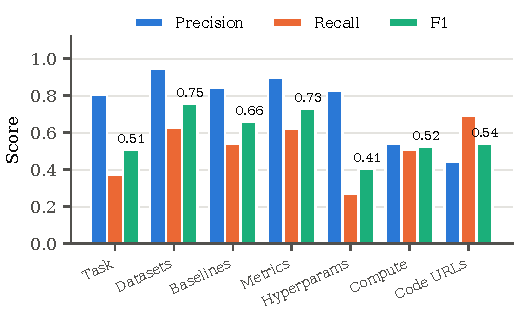
\includegraphics[width=\columnwidth]{figs/fig_fields.pdf}
\caption{Precision, recall and F1 per field. Precision is close to 1 everywhere, and recall
limits F1.}
\label{fig:fields}
\end{figure}

Fig.~\ref{fig:papers} breaks F1 down by paper. Hyperparameter recall is lowest for papers
that put their settings in appendix tables (LoRA: F1~0.06) or that list several model
sizes (Transformer, BERT, DistilBERT). Task F1 is zero for DistilBERT and LoRA because
their extracted tasks were stated more generally than the gold.

\begin{figure}[t]
\centering
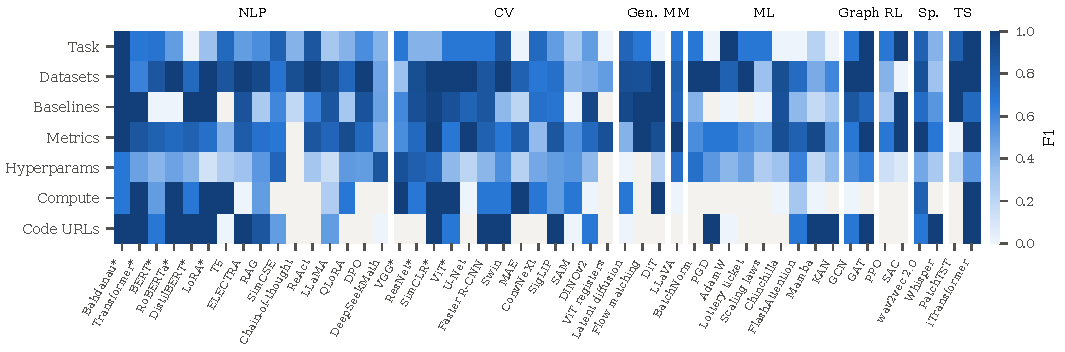
\includegraphics[width=\columnwidth]{figs/fig_papers.pdf}
\caption{Per-paper F1 by field (``--'': no gold code URL for that paper). Hyperparameters
in appendix tables (LoRA) are the main failure.}
\label{fig:papers}
\end{figure}

\subsection{Evidence policy (ablation A3)}
Because every item carries a status, we can score the same extraction under stricter
evidence policies without new LLM calls (Fig.~\ref{fig:a3}). Requiring the quote to be
found in the paper lowers the hallucination rate from 10\% to 2\%. Additionally requiring
the support check (supports or partly supports) lowers it to 0\%, while precision stays at
0.96 to 0.97. The cost is recall, which falls from 0.54 to 0.43 under the strictest policy,
because some correct items come with a paraphrased quote that cannot be located. We
therefore keep all items in the interface and badge their status. The reader sees the
evidence level, and the metrics still count every item.

\begin{figure*}[t]
\centering
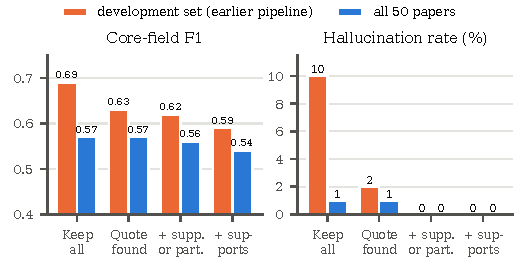
\includegraphics[width=0.92\textwidth]{figs/fig_a3.pdf}
\caption{Ablation A3: the same extraction under four evidence policies (core fields). Left:
precision, recall and F1. Right: hallucination rate. Requiring a located, supporting quote
removes hallucinated items at a moderate cost in recall.}
\label{fig:a3}
\end{figure*}

\subsection{Parser (ablation A1) and retrieval (ablation A6)}
Fig.~\ref{fig:a1} compares GROBID with a PyMuPDF-only parse by the share of gold values
still present in the parsed text, which is an upper bound on extraction recall. Raw
PyMuPDF text keeps slightly more of the values (93\% vs 89\%), mostly numbers in tables
and footnotes. GROBID, however, recovers the structure the rest of the pipeline depends
on: 260 vs 181 section headings, 463 vs 344 references, 67 vs 30 equations, and in-text
citations. With GROBID, 23\% of gold hyperparameter values are absent from the parsed
text, so no prompt change can recover them. For chat, BM25 alone finds the passage holding
a gold answer in its top five for 47\% of questions built from the gold set. The dense and
hybrid arms are pending (Section~\ref{sec:limits}).

\begin{figure}[t]
\centering
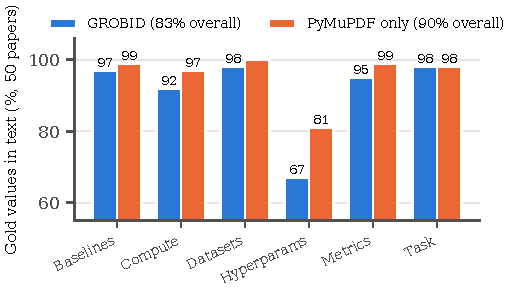
\includegraphics[width=\columnwidth]{figs/fig_a1.pdf}
\caption{Ablation A1: gold values still present in the parsed text, by field (unlabelled
bars are 100\%).}
\label{fig:a1}
\end{figure}

\subsection{Reproducibility, code and other checks}
Table~\ref{tab:phases} summarises the acceptance checks of the other components. The
scorecard agreed with the team's annotations on 158 of 210 checklist decisions (75\%,
$\kappa = 0.57$). This is below the targets of 80\% and $\kappa = 0.6$, but up from 65\%
before item-level guidance was added. The largest disagreements concern training time,
re-run baselines and README instructions. Repository discovery found the official code for
all eight papers that have it.

\begin{table}[t]
\caption{Acceptance checks of the remaining components.}
\label{tab:phases}
\centering
\footnotesize
\setlength{\tabcolsep}{3pt}
\begin{tabular}{@{}p{20mm}p{26mm}p{30mm}@{}}
\toprule
Component & Criterion & Result \\
\midrule
Parsing & 10 arXiv papers; tables on $\geq 8$ & 10/10 \\
Extraction & full output $\leq$ 3 min & 10/10; 15--50 s per paper \\
Repro.\ scorecard & $\geq$ 80\% agreement & 75\%, $\kappa=0.57$ (below target) \\
Code discovery & $\geq$ 80\% repos found & 8/8 \\
Paper vs code & one real mismatch & BERT (below) \\
Chat / math / context & cited answers; glossary on 5 papers; graph & passed (VAE, Adam, DDPM, Transformer, LoRA) \\
\bottomrule
\end{tabular}
\end{table}

\textbf{Case study: BERT.} The paper states that pre-training used a learning rate of
$10^{-4}$, a batch size of 256 and 1M steps~\cite{devlin2019bert}. The static scan of the
official repository found the defaults of \texttt{run\_pretraining.py} to be
$5\times10^{-5}$, 32 and 100{,}000. PaperLens reports this as a mismatch and shows the
paper's sentence beside the code location. The difference is legitimate, since the script's
values are command-line defaults, but anyone running the script as is would not reproduce
the paper. This is exactly the gap the check is meant to surface.

The phase-5 check covered five math-heavy papers (VAE~\cite{kingma2014vae},
Adam~\cite{kingma2015adam}, DDPM~\cite{ho2020ddpm}, Transformer, LoRA). Chat answers cited
pages, off-topic questions were refused, every glossary symbol's quote was verified, and
the citation graph rendered.

\subsection{Interface}
Fig.~\ref{fig:ui} shows the workspace. Clicking an evidence chip scrolls the PDF to the
quoted sentence and highlights it in the colour of its status. Fig.~\ref{fig:compare} shows
the comparison matrix, built from the stored extractions of two papers without an LLM call.
Each cell gives the page where the paper states the item.

\begin{figure*}[t]
\centering
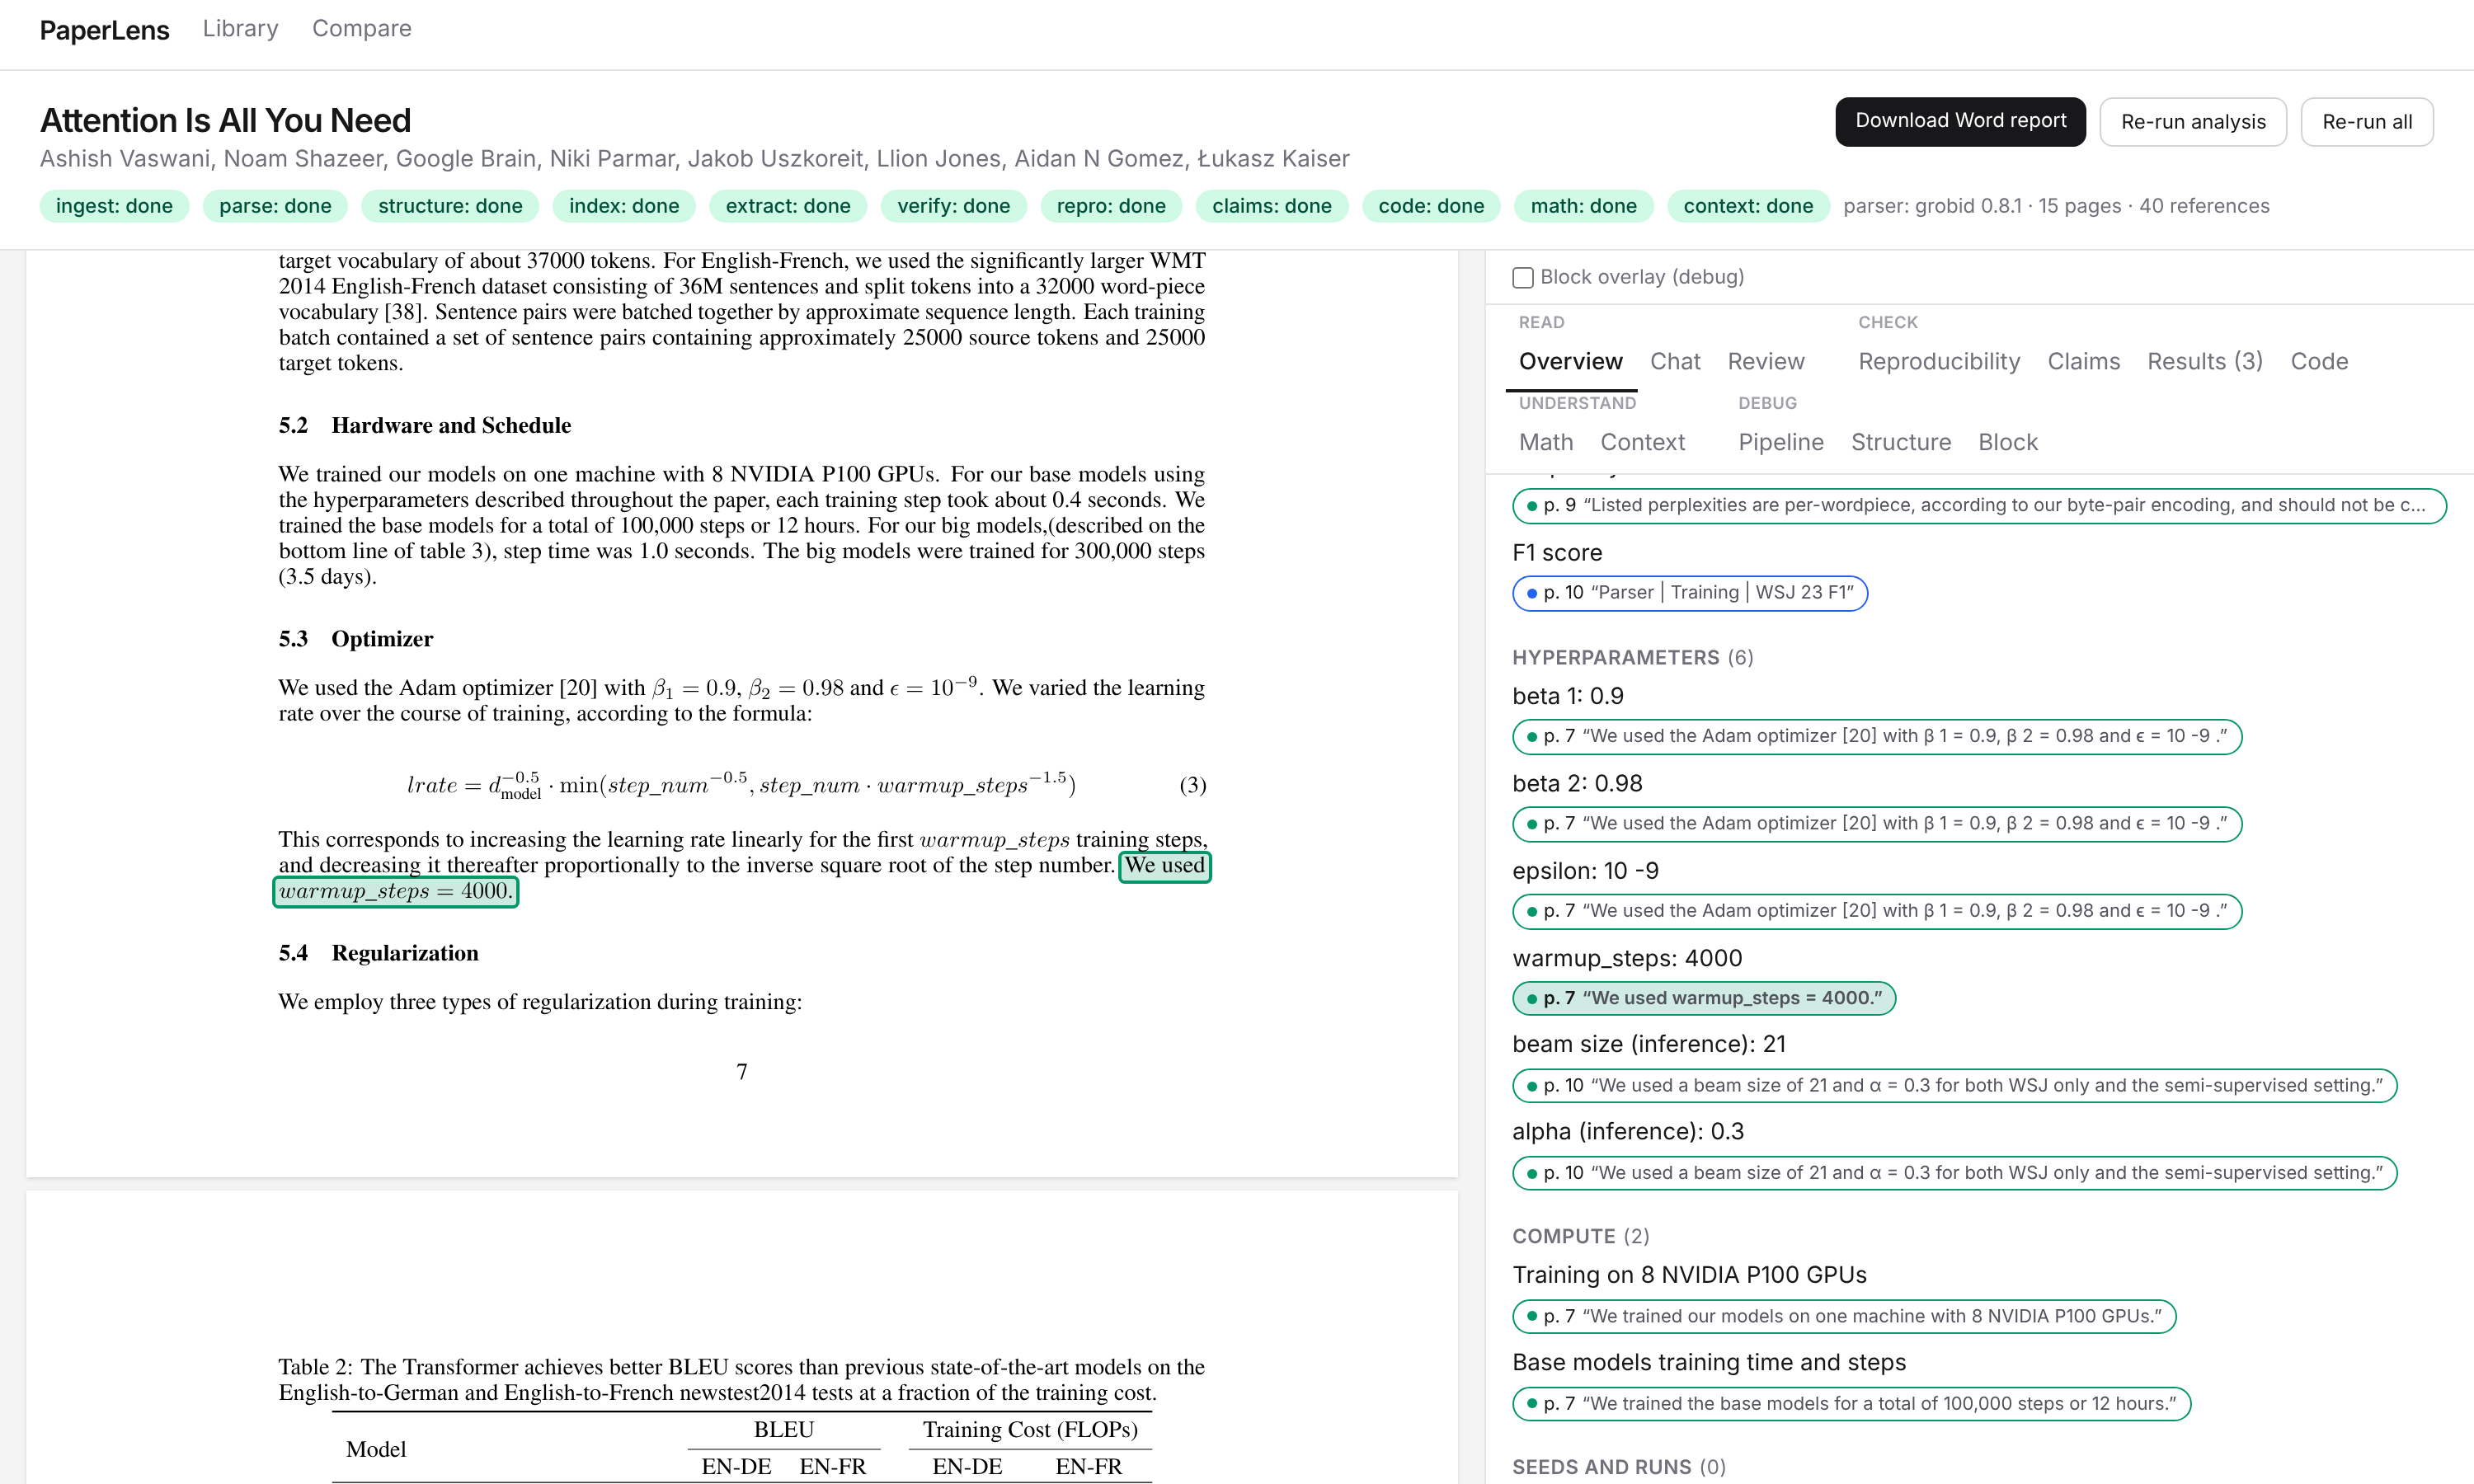
\includegraphics[width=0.95\textwidth]{figs/ui_overview.png}
\caption{The PaperLens workspace on the Transformer paper~\cite{vaswani2017attention}, with
items from the evaluated Gemini run. Selecting the evidence for
\texttt{warmup\_steps: 4000} highlights the source sentence on p.~7 (left). Chip colours
encode the evidence status (green = verified, blue = unchecked).}
\label{fig:ui}
\end{figure*}

\begin{figure}[t]
\centering
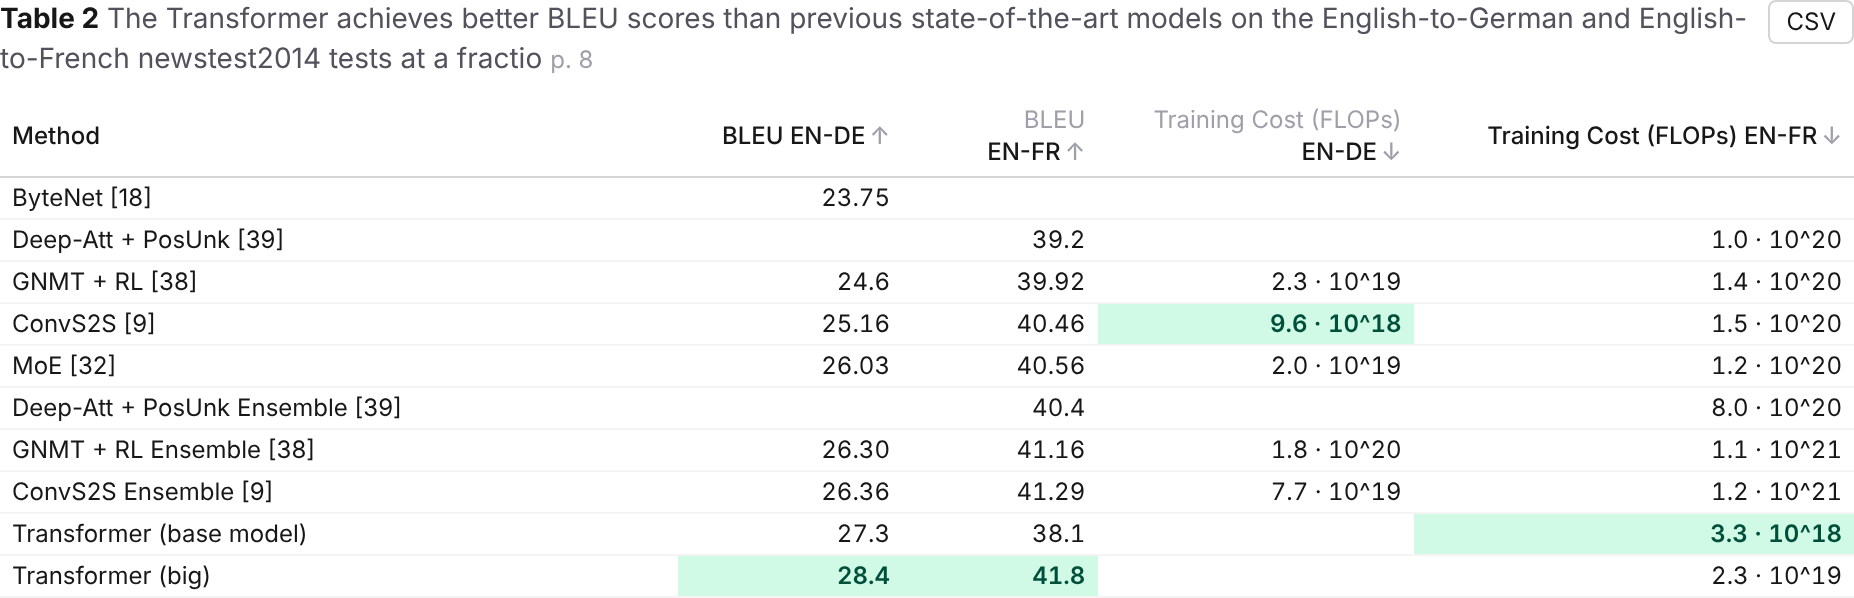
\includegraphics[width=\columnwidth]{figs/ui_results.png}
\caption{A results table rebuilt from word positions (Transformer, Table~2). The best value
per column is computed in Python from the header's direction (higher BLEU and lower
training cost are better).}
\label{fig:results}
\end{figure}

\begin{figure}[t]
\centering
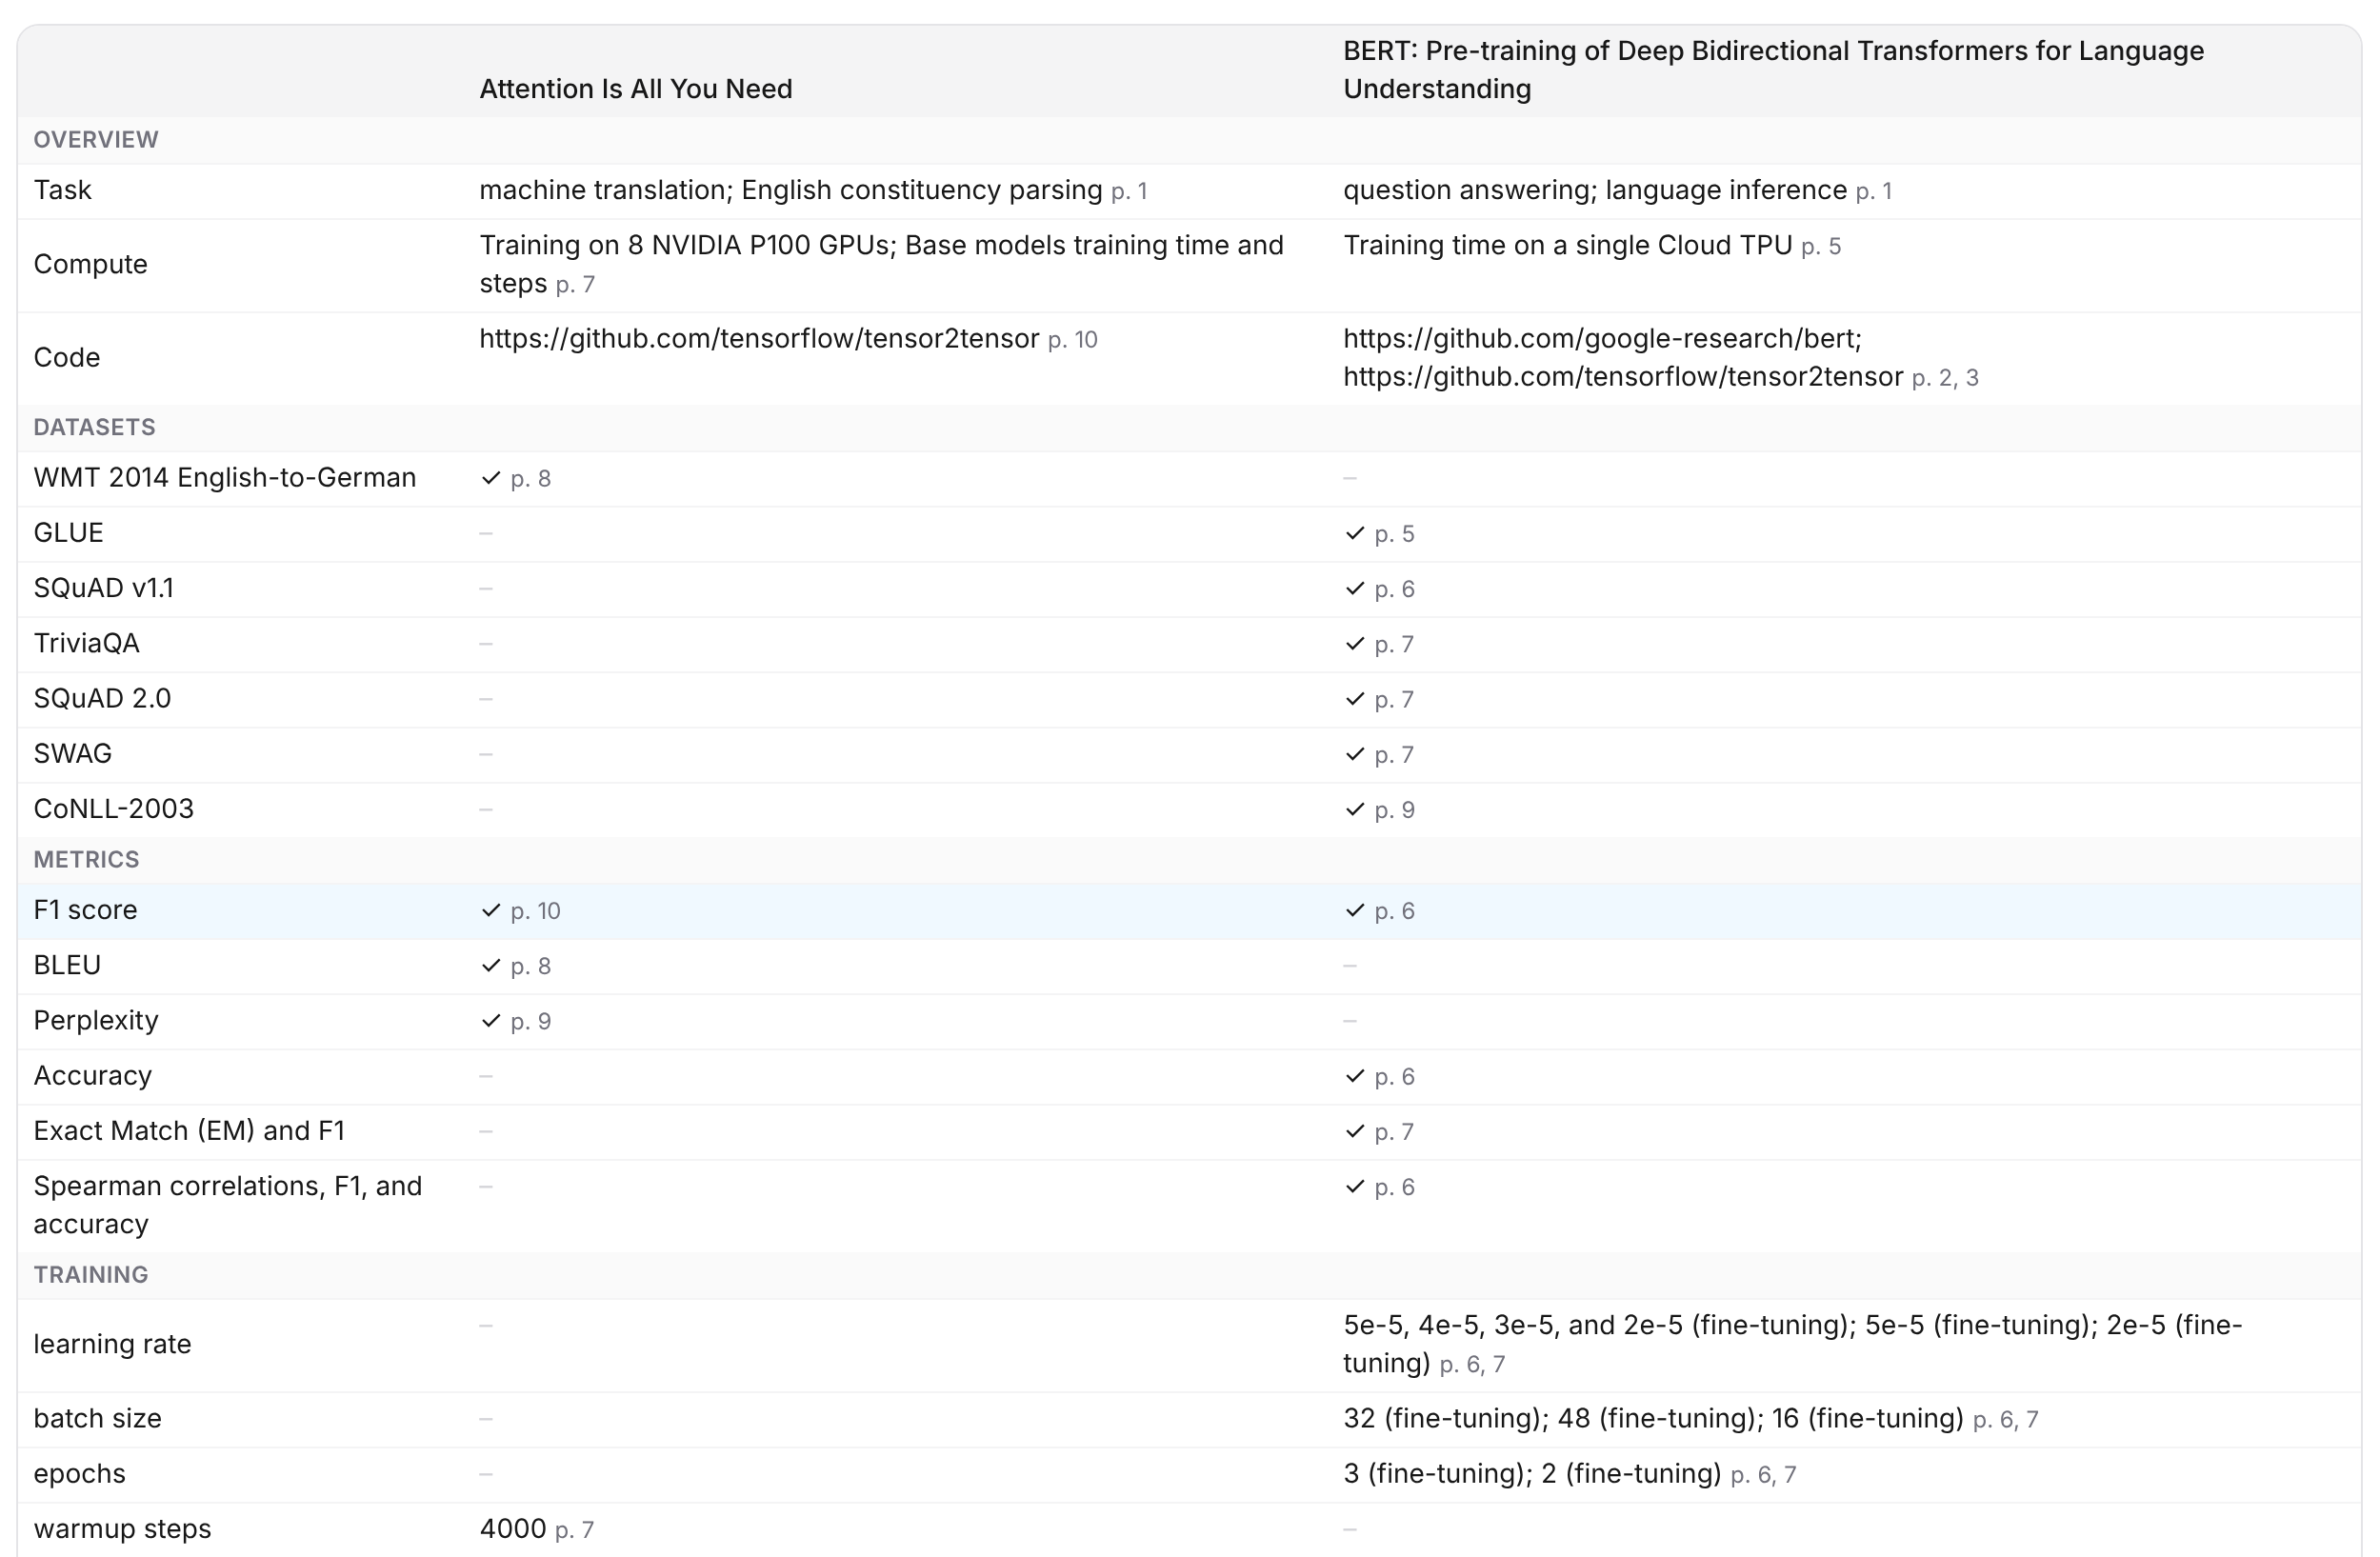
\includegraphics[width=\columnwidth]{figs/ui_compare_crop.png}
\caption{Comparison matrix for two papers (excerpt): tasks, compute, code, datasets and
metrics with the page each is stated on. Rows shared by both papers are tinted.}
\label{fig:compare}
\end{figure}

% =========================================================================================
\section{Error Analysis}

The run missed 214 gold items and produced only 8 items that match nothing in the gold
(Fig.~\ref{fig:errors}). We observe five recurring causes:
\begin{enumerate}
\item \textbf{Appendix and table hyperparameters (dominant).} Of the misses, 130 are
  hyperparameters. An example is Bahdanau et al.'s embedding size 620, maxout size 500 and
  gradient clipping at 1, all in the appendix. Asking for a quote per item seems to favour
  prose over tables, and long appendix groups dilute attention~\cite{liu2024lost}.
\item \textbf{Tasks listed too narrowly.} The model names one or two tasks, whereas the gold
  lists every task the experiments address (for example, VGG's localisation experiments).
\item \textbf{Baselines cited by author name only,} such as transfer-learning comparisons
  given as ``Chatfield et al.\ 2014''. Our scorer also undercounts one case: ``Krizhevsky
  et al.''\ does not match ``Krizhevsky et al.\ 2012'' because digit sequences must be
  equal.
\item \textbf{Wrong code link.} For BERT, a third-party library link was also reported.
  For ViT, a different repository's URL was reported, with the next word glued onto it by
  the PDF text layer.
\item \textbf{Parsing ceiling.} 11\% of gold values do not survive GROBID's text at all
  (A1).
\end{enumerate}

\begin{figure}[t]
\centering
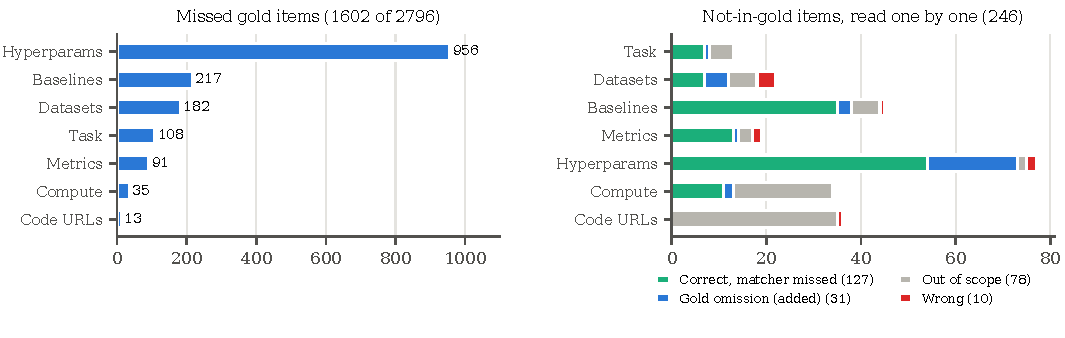
\includegraphics[width=\columnwidth]{figs/fig_errors.pdf}
\caption{Top: missed gold items by field. Bottom: evidence status of all extracted items.}
\label{fig:errors}
\end{figure}

% =========================================================================================
\section{Discussion and Limitations}\label{sec:limits}

\textbf{Precision by construction, recall by effort.} Making the LLM quote its sources, and
checking every quote in code, yields near-perfect precision and a measurable hallucination
rate that can be driven to zero. Recall, however, depends on the model reading every table
and appendix. Table-aware extraction of appendix settings is the most promising next step.

\textbf{Deterministic decisions.} Scores, deltas, verdicts and code comparisons are
computed in Python. They are reproducible, testable with unit tests, and conservative by
design: an ambiguous table match yields ``unsupported'', never ``contradicted''.

\textbf{Limitations.}
\begin{itemize}
\item The gold set is small: 10 papers instead of the planned 40, with no double
  annotation.
\item The scorecard's agreement with the team is below target.
\item Cloning repositories failed on the team's Windows machines, so the code comparison
  was demonstrated on Linux. Repository discovery itself needs no clone.
\item Semantic Scholar often rate-limits, and the context view then falls back to a
  PDF-only citation graph.
\item Several planned ablations are pending:
  \begin{itemize}
  \item extraction granularity (A2);
  \item rule hints (A4);
  \item a stronger model (A5);
  \item LLM vs Python claim verdicts (A7);
  \item extraction without quotes (full A3);
  \item dense and hybrid retrieval (A6);
  \item LaTeX and Docling parsers (A1);
  \item Qasper~\cite{dasigi2021qasper}.
  \end{itemize}
\end{itemize}

\subsection{Threats to validity}\label{sec:threats}
The reference annotations were produced with an LLM and adjudicated once against this
system's output. Where the annotating LLM and Gemini share blind spots, recall may be
overestimated. Where the matcher is strict, as in the digit rule above, it may be
underestimated. Adjudication only added items and never removed any to favour the system,
and every change is logged. A human spot-check of two or three papers is in progress
(TEAM: report the outcome). All results come from a single run of one model, the papers
are well-known ML papers whose text the LLM may have seen in training, and absolute
numbers may not transfer to recent or out-of-domain papers.

\section{Ethics and Privacy}
Paper text is sent to a free-tier API whose inputs may be used to improve the provider's
models. The interface warns users not to upload unpublished or confidential papers.
Repository code is never executed. Reviewer mode gives no score, labels its output as an
LLM draft, and separates it from facts computed in Python, consistent with evidence that
LLM reviews should support human reviewers rather than replace
them~\cite{liang2024feedback,zhou2024reliable}.

\section{Conclusion}
PaperLens shows that a free-tier LLM can support careful paper reading when it is asked
only to extract and quote, while deterministic code locates every quote and makes every
decision. On ten papers it extracts with near-perfect precision and full numeric accuracy
on matched hyperparameters. Every item is traceable to a highlighted sentence, and
requiring evidence eliminates hallucinated items. Future work will target recall on
appendix tables, complete the pending ablations, and extend the gold set with independent
human annotation.

\section*{Acknowledgment}
% TEAM: guide / institution acknowledgement.
The authors thank their project guide for feedback. PaperLens uses GROBID, PyMuPDF and the
Gemini API free tier.

\bibliographystyle{IEEEtran}
\bibliography{refs}

\end{document}
